\documentclass{article}

\usepackage[a4paper, margin=1in]{geometry}
\usepackage{graphicx}
\usepackage{caption}
\usepackage{float}
\usepackage[utf8]{inputenc}
\usepackage[brazil]{babel}

\graphicspath{ {./images/} }
\captionsetup{font=small}

\title{Informação Profissional em Ciência da Computação:\\
       Arquitetura de Computadores}
\author{Carlos Eduardo Gallo Filho \\
        Caio Uehara Martins\\
        Pedro Henrique Mendes de Lima}

\date{\today}

\begin{document}

\maketitle

\section{Introdução}
\subsection{Arquitetura e Organização}
\subsection{Estruturas e Funções}
\subsubsection{Múltiplos núcleos}
\subsubsection{Estrutura interna do núcleo}

\section{Evolução histórica}
\subsection{Primeira geração: Arquitetura de Von Neumann}
A primeira geração de computadores é conhecida pelo uso das válvulas para
representar os elementos lógicos digitais e a memória. E também, o
\textbf{conceito de programa armazenado}, atribuída ao matemático John Von
Neumann, que surgiu para a construção do computador EDVAC (Eletronic Discrete
Variable Computer), mas foi principalmente discutido no desenvolvimento do
computador IAS, o qual é um protótipo para quase todos os computadores de
propósito geral de hoje em dia.

\begin{figure}[h]
    \centering
    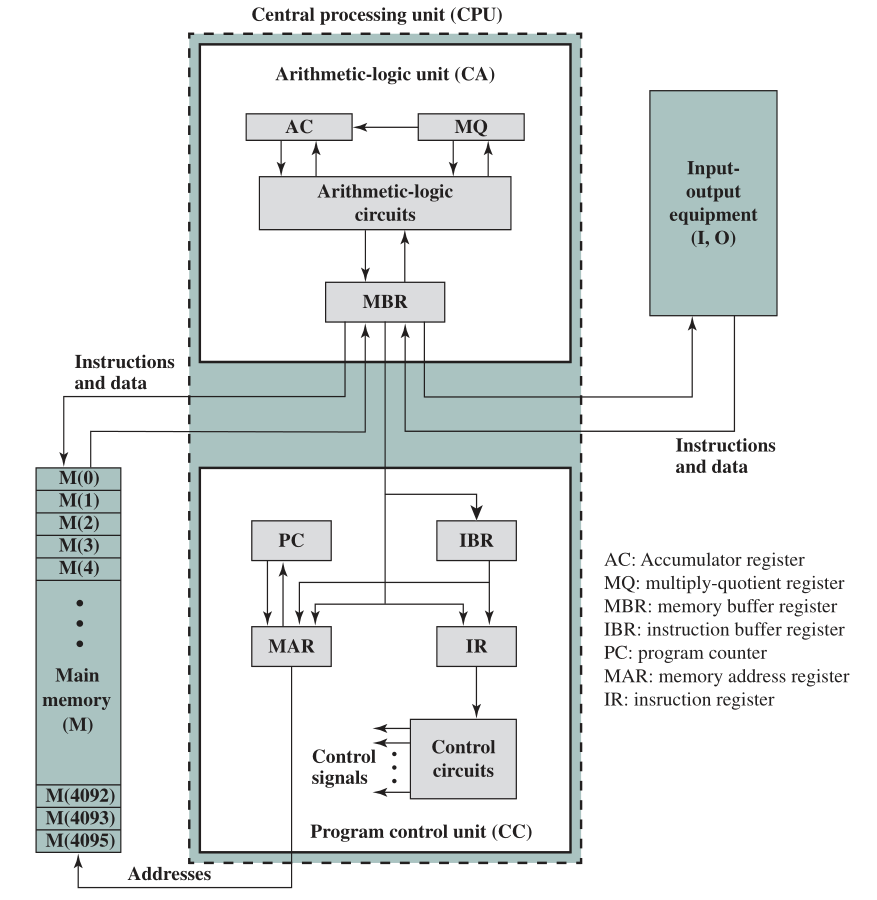
\includegraphics[width=0.65\textwidth]{ias.png}
    \caption{Estrutura do IAS.}
\end{figure}

Para se explicar a estrutura do IAS, deve-se atentar a 5 partes principais:

\begin{enumerate}
    \item Um computador terá de ser capaz de executar as operações elementares
        básicas (adição, subtração, multiplicação, divisão). Normalmente, para
        essas funções são criadas unidades específicas para tais, comportadas em
        uma unidade maior centralizadora denominada CA ou unidade lógica e
        aritmética.

    \item Um computador terá de ser capaz de dar sequenciamento adequado as suas
        operações, instruções e as instruções de controle (comandos que regem o
        próprio sequenciamento do computador). Á essas unidades é denominada uma
        unidade central chamada CC ou controle central.

        As partes 1) e 2) juntas são chamadas de C. 

    \item Um computador terá a necessidade de processar sequências longas de
        operações, que, geralmente, não conseguem ser efetuadas em uma única
        leva de comandos. Logo, requer-se uma unidade que armazene dados por
        períodos duráveis para resolver problemas mais complexos, como cálculos.

        Essa unidade é denominada M ou memória.

        Analogamente ao funcionamento do corpo humano, essas três partes podem
        ser comparadas a parte cognitiva do corpo. Ou seja, a unidade lógica e
        aritmética, o controle central e a memória são o conjunto pensante do
        computador. Mas, assim como o corpo humano, se faz necessário a
        comunicação com o mundo externo, tal é feito por um canal denominado
        meio de gravação de saída do dispositivo ou R, de modo que as últimas
        duas partes interagem com esse canal para satisfazer a necessidade de
        interação com o externo. 

    \item A parte de entrada do meio R, a qual deve transferir as informações
        desse para dentro de M e C é chamada de entrada ou I. É de boa prática a
        entrada passar os dados para dentro de M e nunca diretamente para C. 

    \item Similarmente, a parte de saída do meio R, a qual deve transferir as
        informações de M e C para o meio R, é chamada de saída ou O. É de boa
        prática, também, a saída passar de M para R, assim, nunca diretamente
        por C. 
\end{enumerate}

Assim, resumidamente, temos a memória principal, que armazena dados e
instruções; a unidade lógica e aritmética (ALU), que opera os binários; a
unidade de controle, que interpreta e executa instruções e, por fim, o
equipmaneto de saída (E/S), que conecta o meio interno ao meio externo do
computador.

Como já antes dito, o modelo de IAS reflete em grande parte dos computadores
atuais, por isso sua importância no mundo da computação.

\subsubsection{Endereçamento de memória}
O IAS possui 4.096 locais de armazenamento chamados de palavras, sendo esses
dados ou instruções, cada um com 40 bits. As palavras são dividas em duas:
palavra de número e palavra de instrução.

\begin{itemize}
        \item Palavra de número: contém um bit de sinal e outros 39 de
            armazenamento para o número. 
        \item Palavra de instrução: pode conter duas instruções de 20 bits,
            cada uma contendo um opcode de 8 bits - referência que um
            processador possui para uma determinada instrução - e 12 bits de
            endereço de memória.
\end{itemize}

\begin{figure}[H]
   \centering
   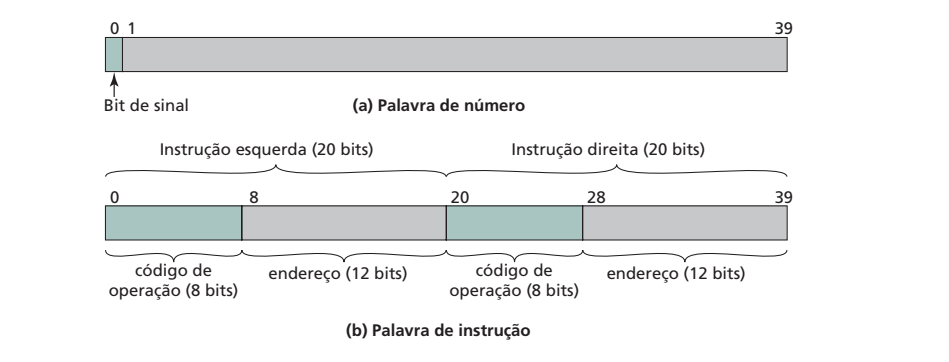
\includegraphics[width=0.75\textwidth]{palavras.png}
   \caption{Tipos de palavras de memória.}
\end{figure}

\subsubsection{Registradores}
Passando para as unidades menores do computador IAS, tem-se os locais de
armazenamento da unidade de controle e da ALU, chamados de registradores.

\begin{itemize}
    \item \textbf{Registrador de buffer de memória (MBR):} é o local onde permanece
            a palavra a ser armazenada na memória ou enviada à unidade E/S,
            como também é o local para receber a palavra a partir da E/S ou a
            partir da memória.
        \item \textbf{Registrador de endereço de memória (MAR):} local que contém o
            endereço da memória da palavra a ser escrito ou lido pelo MBR.
        \item \textbf{Registrador de instruções (IR):} contém o opcode de 8 bits da
            instrução que está sendo executada.
        \item \textbf{Registrador de buffer de instrução (IBR):} mantém temporariamente
            a instrução da direita da palavra da memória.
        \item \textbf{Contador do programa (PC):} mantém o próximo par de instruções a
            ser buscado na memória.
        \item \textbf{Acumulador (AC) e quociente-multiplicador (MQ):} registradores
            usados para realizar as operações da ALU, sendo o AC o que mantém
            os bits mais significativos e o MQ os bits menos significativos.
\end{itemize}

\subsubsection{Ciclos do IAS}
\subsubsection{Conjunto de instruções IAS}
\subsection{Segunda geração: Transístores}
\subsection{Terceira geração: Circuitos Integrados}
\subsection{Gerações posteriores}
\subsection{Comparação entre as gerações}

\section{Aplicações} 
As subseções a seguir trazem algumas aplicações da arquitetura de computadores.
\subsection{Paradigmas de arquitetura}

\subsubsection{CISC}
O paradigma de arquitetura CISC (\textit{Complex Instruction Set Computer})
denotam uma escolha de projeto na qual o conjunto das instruções utilizadas são
projetadas para a execução de um conjunto de operações de baixo nível,
envolvendo por exemplo, operações aritméticas juntas de uma escrita na memória,
tudo em uma mesma instrução.

Uma notória vantagem do uso do paradigma CISC se dá por facilitar a construção
de compiladores e a programação em baixo nível, pois as instruções fornecem um
pequeno nível de abstração. Além disso, por implementar as instruções a comuns
nível de \textit{hardware}, o consumo de memória, tempo de execução e tamanho dos
programas costumam ser menores. Uma desvantagem direta ao paradigma é o fato do
projeto do hardware se tornar muito mais trabalhoso e complexo, além de
necessitar maior quantidade de componentes, e por consequência, aumento de
calor.

\subsection{RISC}
Em contrapartida ao CISC, existe o paradigma RISC (\textit{Reduced Instruction
Set Computer}). Um projeto RISC tem como princípio implementar um pequeno número
mínimo de instruções simples, que em sua maioria são executadas em apenas um
ciclo de máquina.

Como esperado, processadores RISCs são mais fáceis de serem implementados e
produzidos, gastando menor quantidade de componentes e melhorando a eficiência
térmica, além de facilitar a implementação do \textit{pipelining} a nível do
código de máquina. Como desvantagem, sua programação de baixo nível é mais
complexa, bem como a construção de compiladores, o que implica uma má
implementação a nível de software ser mais danosa.

\subsection{Arquitetura x86} 
A arquitetura de processadores x86 foi concebida pela intel e é o exemplar mais
popular do tipo CISC, trazendo muitos princípios de \textit{design} que só
existiam até então em \textit{mainframes}. A arquitetura teve seu surgimento
junto ao processador 8086 em 1978, que foi introduzido como uma extensão de 16
bits ao famoso 8080, primeiro microprocessador de propósito geral.

A linhagem de processadores x86 continuou a evoluir, levando ao aparecimento do
80286, 80386 e 80486, cada qual incrementando novas instruções na arquitetura,
além de melhorar aspectos de organização utilizando a rápida evolução da
microeletrônica. O 80286 possibilitou a ampliação do número de memória
endereçável para 16 MB, ao invés de 1 MB que seu antecessor era capaz. Já o
80386 foi o primeiro processador de 32 bits, trazendo muitas melhorias em
comparação ao 80236, o que inclui o suporte a multitarefas. Sucessivamente, o
80486 incrementou uma nova tecnologia de cache junto de uma avançada
\textit{pipelining} de instruções, além de também adicionar um coprocessador
para instruções matemáticas complexas.

Já entrando na quinta geração de processadores, surge o Pentium, que sucede o
80486 adicionando tecnologia superescalar, que é uma forma de paralelismo a
nível de instrução utilizando múltiplas unidades de execução. Seguindo para o
Pentium Pro, este continuou a implementação de técnicas multi-escalares,
incluindo análise do fluxo de dados, execução especulativa, entre outras.

Com os desktops se tornando cada vez mais comuns e novas necessidades surgindo,
levando ao aparecimento de instruções orientadas ao processamento de multimídia.

O Pentium II surge incorporando a tecnologia MMX da Intel no Pentium Pro. Em
seguida, o Pentium III trouxe muitas outras novas instruções de ponto flutuante,
que melhoravam muito a performance em algumas aplicações específicas. O ultimo
processador da linha foi o Pentium 4, que apenas melhorou algumas tecnologias
utilizadas em seu antecessor.

Após a virada do século, o desenvolvimento de novos processadores acabou mudando
de rumo, quando foi alcançado limites práticos para o aumento do \textit{clock},
por exemplo. Como não era possível mais aproveitar os avanços da miniaturização
para melhorar a performance, os processadores passaram a serem multiplicados em
diferentes núcleos. O primeiro \textit{dual core} x86 foi o Intel Core.
Posteriormente o Intel Core foi estendido a 64 bits, surgindo posteriormente
variantes como o Core 2 Quad, com quatro nucelos. Outra tecnologia importante
adicionada à linha Core 2 foram as AVE, que possuíam instruções de grande
tamanho para processamento eficiente de vetores.

Por mais que a arquitetura x86 seja antiga, ela se mostrou em constante
evolução, o que inclui sempre a adição de novos recursos e instruções,
aproveitando os avanços da microeletrônica para mudanças na organização. Ainda
assim, processadores recentes possuem retrocompatibilidade com programas
antigos, devido ao fato da arquitetura ter evoluído sem alterar instruções já
existentes, o que colaborou para a manutenção da popularidade da arquitetura.

\subsection{Sistemas embarcados}
Sistemas embarcados são caracterizados pela combinação de \textit{hardware} e
\textit{software} utilizados em conjunto para formar um sistema de propósito
específico, em contraste aos computadores de propósito geral abordados. Os tipos
de sistemas embarcados são dos mais variados, incluindo desde sistemas
automotivos até telefones celulares.

A organização de um sistema embarcado, como esperado, também difere à de um
sistema de propósito geral, o que inclui partes estritamente planejadas para o
ambiente de trabalho do sistema. Isso implica que no geral, sistemas embarcados
diferem muito entre si, e portanto são difíceis de serem caracterizados de
maneira genérica. No entanto, algumas características comuns de sistemas
embarcados podem ser descritas:

\begin{figure}[h]
    \centering
    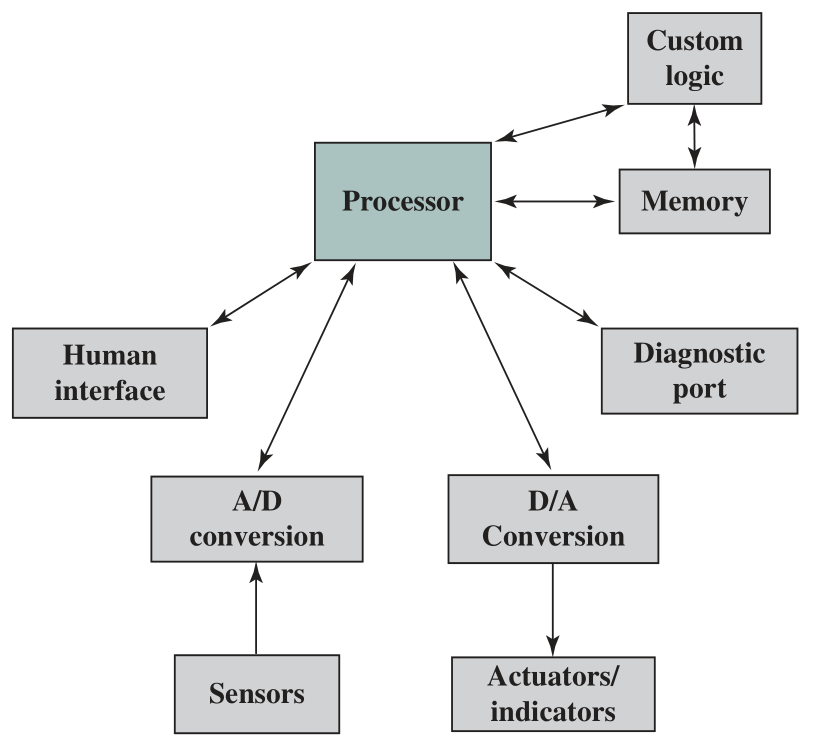
\includegraphics[width=0.4\textwidth]{embarcado.png}
    \caption{Possível organização de um sistema embarcado}
\end{figure}

\begin{itemize}
    \item Possuem uma interface de comunicação com o ambiente,
        o que inclui sensores integrados.

    \item A interface de usuário é simplificada, sendo até mesmo
        inexistente em alguns projetos.

    \item A interface de depuração muitas vezes é utilizada para
        diagnostico do sistema controlado, não apenas do microcontrolador.

    \item Uso de hardware especializado, incluindo até mesmo circuitos
        não digitais em alguns casos.

    \item Software possui uma função e objetivo fixo e bem definido.

    \item Eficiência é de extrema importância, o que inclui performance,
        baixo consumo de energia, espaço e consumo de memória.
\end{itemize}

Alguns sistemas embarcados complexos acabam incorporando processadores de
aplicação, capaz de executarem sistemas operacionais complexos, o que inclui a
adição da natureza de propósito geral aos microcontroladores, ainda que em suma
maioria estes possuam apenas um processador dedicado.

\subsubsection{Microcontroladores}
Enquanto microprocessadores se beneficiaram dos avanços da miniaturização de
componentes aumentando seu conjunto de instruções, memória e núcleos, os
microcontroladores o usam para integrar todos os outros componentes de um
computador em um único chip, o que inclui memória RAM, ROM, \textit{clock} e
unidade de controle de entrada e saída. Obviamente, os elementos de um
microcontrolador são mais simples, porém possuem alta eficiência energética e
baixíssimo custo.

\begin{figure}[h]
    \centering
    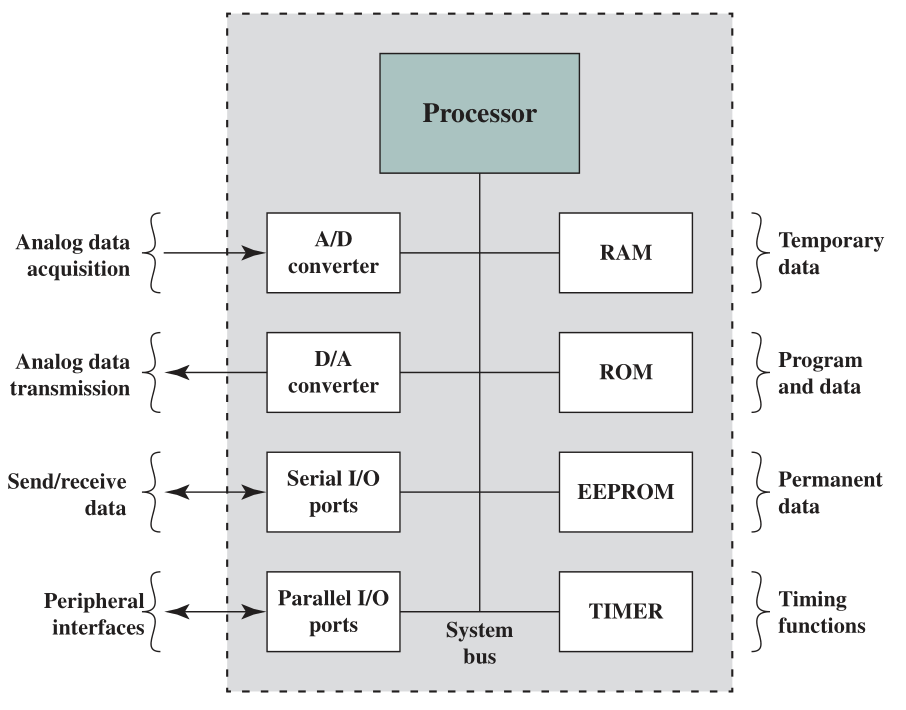
\includegraphics[width=0.6\textwidth]{uc.png}
    \caption{Organização típica de um microcontrolador}
\end{figure}

\subsubsection{Internet das Coisas (IoT)}
O termo IoT (\textit{Internet of Things}) é utilizado para denotar o fenômeno de
expansão da rede de comunicação entre dispositivos embarcados "inteligentes". O
fenômeno vem se tornando cada vez mais popular e denota a inclusão de sistemas
micro-controlados em objetos dos mais variados tipos, como geladeira, lampadas e
torradeiras. a IoT é responsável pela integração dos possíveis objetos para
formar um grande sistema automatizáveis. Um exemplo clássico de IoT são os
sistemas de automação residencial.

Uma caraterística importante dos sistemas IoT é o caráter da conexão dos seus
principais dispositivos, definida por baixa largura de banda, baixa repetição de
captura e uso de dados.

\subsection{Arquitetura ARM} 
A família de arquitetura ARM é caracterizada por uma grande gama de
microprocessadores e microcontroladores, sendo a exemplar mais popular do tipo
RISC. Diferente da arquitetura x86, a empresa por trás da arquitetura ARM não
fabrica processadores, mas sim os projeta, além de projetar também a arquitetura
em si, vendendo licenças de fabricação às fabricantes.

Como consequência do paradigma RISC, os chips ARM possuem tamanho reduzido e
baixíssimo consumo energético, principalmente pela pequena quantidade de
componentes necessários. Essas características levam os microprocessadores ARM a
dominarem o mercado de dispositivos móveis, como o de \textit{smartphones}.

O conjunto de instruções ARM é desenvolvido para eficiente implementação e
execução. Todas instruções são de 32 bits e seguem formato regular, permitindo
sua implementação em uma vasta gama de produtos. Além disso, ainda existe o
conjunto de instruções \textit{Thumb}, que é um subconjunto do conjunto de
instruções ARM tradicionais, cujas instruções são implementadas em 16 bits para
melhor performance e menor largura de barramento de memória, permitindo
consequentemente melhor densidade de código.

Talvez uma das principais famílias de microprocessadores ARM sejam os da linha
Cortex, que são nomeados de acordo com suas respectivas aplicações. O Cortex-A
e o Cortex-A50 são processadores de aplicação, ou seja, são capazes de rodar sistemas
operacionais completos, sendo utilizados em smartphones, por exemplo. Já o
Cortex-R é projetado para aplicações embarcadas de baixa latência, contendo
otimizações tanto em seu conjunto de instrução quanto sua organização para
melhor desempenho. Por ultimo, existe a série Cortex-M, que é desenvolvida
princialmente para o domínio de microcontroladores.

O ARM Cortex-M3 por exemplo, que é utilizado para microcontroladores de 16 e 32
bits, contando com funcionalidades de \textit{debug} e \textit{trace}. Uma
diferença relatável do Cortex-M3 é que ele utiliza barramentos diferentes para
instruções e dados, que difere do IAS, por exemplo, e que torna possível ler
ambos barramentos ao mesmo tempo, oferecendo paralelismo. Além disso, possui um
decodificador \textit{Thumb}, uma avançada ULA (Unidade Lógica e Aritmética)
com suporte à multiplicação e divisão, controle logico e interface com os outros
componentes do processador.

Além do "núcleo" do processador, o Cortex-M3 também possui alguns componentes,
dos quais:

\begin{itemize}
    \item \textbf{NVIC:} Provê gerenciamento de interrupções e controle
        energético.
    \item \textbf{ETM:} Componente de depuração que permite reconstrução da
        execução de programas
    \item \textbf{Debug access port (DAP):} Interface para depuração externa
    \item \textbf{Debug logic:} Fornece funcionalidades básicas de depuração.
    \item \textbf{ICode interface:} Pega as instruções do espaço de memória de
        código
    \item \textbf{SRAM \& peripheral interface:} Interface de leitura e escrita
        de memória e dispositivos externos.
    \item \textbf{Bus matrix:} Conecta o núcleo e a interface de depuração com
        o barramento externo do microcontrolador.
    \item \textbf{Memory protection unit:} Responsável pela proteção de dados
        críticos do sistema operacional. 
\end{itemize}

\begin{figure}[h]
    \centering
    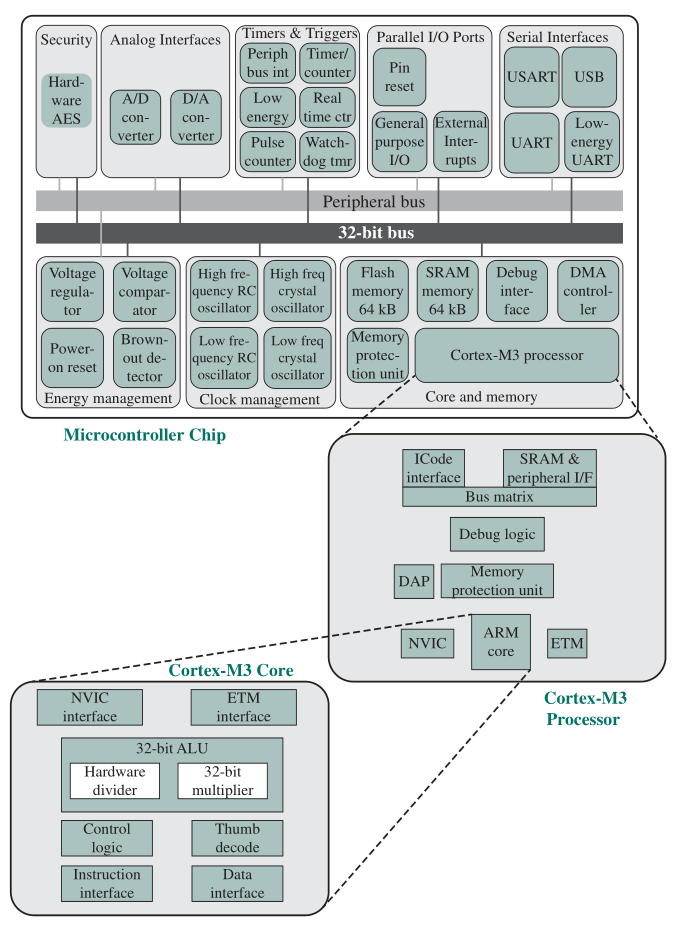
\includegraphics[width=0.8\textwidth]{cortex.png}
    \caption{Típica estrutura de um chip de um microcontrolador baseado no
    Cortex-M3.}
\end{figure}

Já um microcontrolador baseado no Cortex-M3, possui:

\begin{itemize}
    \item \textbf{Core and memory:} Região que inclui o processador, RAM
        estática, memória \textit{flash} e interface de depuração.
    \item \textbf{Parallel I/O ports:} Portas paralelas de I/O configuráveis.
    \item \textbf{Serial interfaces:} Suporte para I/O serial.
    \item \textbf{Analog interfaces:} Conversores A/D e D/A para suporte a
        sensores e atuadores.
    \item \textbf{Timers and triggers:} Responsável por acompanhar eventos de
        contagem e manipulação de tempo, além de gerar formas de ondas e
        gatilhar ações temporais em periféricos.
    \item \textbf{Clock management:} Controla os osciladores e relógios do chip.
    \item \textbf{Energy management:} Gerencia os modos de operação em baixa
        energia.
    \item \textbf{Security:} Implementação do padrão AES \textit{Advanced
        Encryption Standard}.
    \item \textbf{32-bit bus:} Barramento que conecta todos os componentes do
        chip.
    \item \textbf{Peripheral bus:} Barramento que permite interconexão dos
        módulos sem envolver o processador.
\end{itemize}

\subsection{Computação em Nuvem}
Com o avanço das tecnologias de telecomunicações, o que envolve as redes de
computadores, se tornou comum o oferecimento de serviços computacionais
disponíveis pela Internet \textbf{sob demanda}. Tais serviços incluem
armazenamento de arquivos, hospedagem de aplicações, máquinas virtuais, execução
de softwares entre outros. Isso resulta em uma menor complexidade na manutenção
e maior escalabilidade dos sistemas finais.

A justificativa para a existência dos serviços em nuvem é a redução do trabalho
necessário para provisionamento e manutenção de uma infraestrutura de TI para
atividades que envolvem produtos finais pertencentes às camadas mais superiores
da stack de software\footnote{O termo stack de software é utilizado para denotar
os diferentes subsistemas de software que compõe uma plataforma completa.}, pois
esse passa a ser terceirizado a um provedor de nuvem (CSP, do inglês
\textit{Cloud Service Provider}). Os serviços nuvem oferecem portanto uma menor
complexidade para seus usuários, bem como maior escalabilidade.

As modalidades de serviços podem ser divididas em ordem crescente de abstração
em: IaaS (\textit{Infrastructure as a Service}), PaaS (\textit{Plataform as a
Service}) e SaaS (\textit{Software as a Service}). O primeiro se refere ao
fornecimento de uma infraestrutura de hardware virtual, provendo um ambiente
customizável a nível de sistema operacional. Já o segundo, provê um ambiente
para hospedagem de aplicações arbitrárias do usuário, contando com todo o resto
administrado pelo provedor do serviço. Por fim, o Saas se refere ao serviço da
execução de um programa na infraestrutura da provedora.

Ademais as aparentes vantagens, a arquitetura em nuvem apresenta muitos
problemas críticos, como de segurança e privacidade. Atualmente se existe o
oligopólio das \textit{big techs}, cujos serviços principais são pautados na
manipulação, processamento e posse dos dados de seus clientes e usuários. Além
disso, a arquitetura nuvem possui menor flexibilidade quanto ao controle e
conhecimento do usuário sobre as camadas inferiores do sistema.

\nocite{stallings}

\bibliographystyle{plain}
\bibliography{ref}

\end{document}
